\section{Date: 2026-08-29}
\noindent \textbf{Series ID: FWSTHLTHSOCASSRGSP} 

\noindent This series is titled Real Gross Domestic Product: Health Care and Social Assistance (62) in the Far West BEA Region and has a frequency of Annual. The units are Millions of Chained 2017 Dollars and the seasonal adjustment is Not Seasonally Adjusted.The observation start date is 1997-01-01 and the observation end date is 2025-01-01.The popularity of this series is 1. \\ 

\noindent \textbf{Series ID: IEAXIP} 

\noindent This series is titled Primary Income Receipts: Investment income: Portfolio investment income and has a frequency of Quarterly. The units are Millions of Dollars and the seasonal adjustment is Seasonally Adjusted.The observation start date is 1999-01-01 and the observation end date is 2026-01-01.The popularity of this series is 1. \\ 

\subsection{Raw Regression}
\noindent Regresses the two series against each other directly. A significant result here can come just as easily from both series sharing a long-run trend as from any real relationship.

\begin{center}
\begin{tabular}{lclc}
\toprule
\textbf{Dep. Variable:}                  & value\_fred\_IEAXIP & \textbf{  R-squared:         } &     0.966   \\
\textbf{Model:}                          &         OLS         & \textbf{  Adj. R-squared:    } &     0.965   \\
\textbf{Method:}                         &    Least Squares    & \textbf{  F-statistic:       } &     718.1   \\
\textbf{Date:}                           &   Sat, 29 Aug 2026  & \textbf{  Prob (F-statistic):} &  6.19e-20   \\
\textbf{Time:}                           &       15:49:09      & \textbf{  Log-Likelihood:    } &   -275.36   \\
\textbf{No. Observations:}               &            27       & \textbf{  AIC:               } &     554.7   \\
\textbf{Df Residuals:}                   &            25       & \textbf{  BIC:               } &     557.3   \\
\textbf{Df Model:}                       &             1       & \textbf{                     } &             \\
\textbf{Covariance Type:}                &      nonrobust      & \textbf{                     } &             \\
\bottomrule
\end{tabular}
\begin{tabular}{lcccccc}
                                         & \textbf{coef} & \textbf{std err} & \textbf{t} & \textbf{P$> |$t$|$} & \textbf{[0.025} & \textbf{0.975]}  \\
\midrule
\textbf{const}                           &   -5.329e+04  &     4644.132     &   -11.476  &         0.000        &    -6.29e+04    &    -4.37e+04     \\
\textbf{value\_fred\_FWSTHLTHSOCASSRGSP} &       0.5530  &        0.021     &    26.797  &         0.000        &        0.510    &        0.595     \\
\bottomrule
\end{tabular}
\begin{tabular}{lclc}
\textbf{Omnibus:}       &  0.189 & \textbf{  Durbin-Watson:     } &    1.346  \\
\textbf{Prob(Omnibus):} &  0.910 & \textbf{  Jarque-Bera (JB):  } &    0.335  \\
\textbf{Skew:}          &  0.166 & \textbf{  Prob(JB):          } &    0.846  \\
\textbf{Kurtosis:}      &  2.567 & \textbf{  Cond. No.          } & 8.04e+05  \\
\bottomrule
\end{tabular}
%\caption{OLS Regression Results}
\end{center}

Notes: \newline
 [1] Standard Errors assume that the covariance matrix of the errors is correctly specified. \newline
 [2] The condition number is large, 8.04e+05. This might indicate that there are \newline
 strong multicollinearity or other numerical problems.

\begin{figure}
\centering
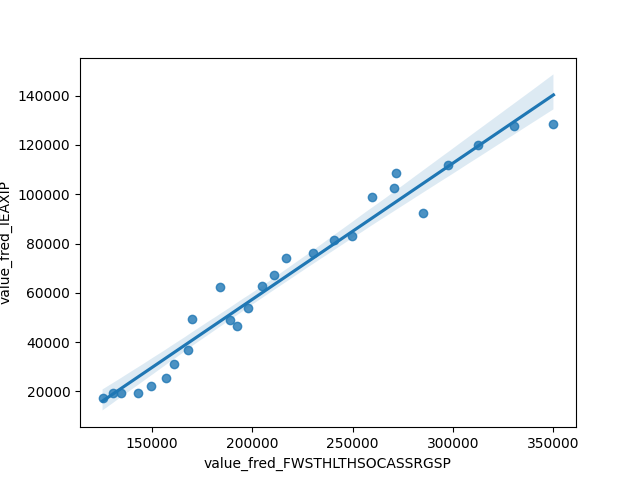
\includegraphics[scale = 0.9]{plots/plot_2026-08-29.png}
\caption{Raw Regression Plot for 2026-08-29}
\end{figure}
\newpage
\subsection{Detrended Regression}
\noindent Regresses the residuals of each series after removing its own linear time trend, so a shared trend can no longer drive the result on its own. A relationship that stays significant here is better evidence of a genuine link between the two series.

\begin{center}
\begin{tabular}{lclc}
\toprule
\textbf{Dep. Variable:}                             & value\_fred\_IEAXIP\_detrended & \textbf{  R-squared:         } &     0.177   \\
\textbf{Model:}                                     &              OLS               & \textbf{  Adj. R-squared:    } &     0.144   \\
\textbf{Method:}                                    &         Least Squares          & \textbf{  F-statistic:       } &     5.362   \\
\textbf{Date:}                                      &        Sat, 29 Aug 2026        & \textbf{  Prob (F-statistic):} &   0.0291    \\
\textbf{Time:}                                      &            15:49:09            & \textbf{  Log-Likelihood:    } &   -272.20   \\
\textbf{No. Observations:}                          &                 27             & \textbf{  AIC:               } &     548.4   \\
\textbf{Df Residuals:}                              &                 25             & \textbf{  BIC:               } &     551.0   \\
\textbf{Df Model:}                                  &                  1             & \textbf{                     } &             \\
\textbf{Covariance Type:}                           &           nonrobust            & \textbf{                     } &             \\
\bottomrule
\end{tabular}
\begin{tabular}{lcccccc}
                                                    & \textbf{coef} & \textbf{std err} & \textbf{t} & \textbf{P$> |$t$|$} & \textbf{[0.025} & \textbf{0.975]}  \\
\midrule
\textbf{const}                                      &   -1.038e-09  &     1156.400     & -8.97e-13  &         1.000        &    -2381.651    &     2381.651     \\
\textbf{value\_fred\_FWSTHLTHSOCASSRGSP\_detrended} &       0.2639  &        0.114     &     2.316  &         0.029        &        0.029    &        0.499     \\
\bottomrule
\end{tabular}
\begin{tabular}{lclc}
\textbf{Omnibus:}       &  0.703 & \textbf{  Durbin-Watson:     } &    1.593  \\
\textbf{Prob(Omnibus):} &  0.704 & \textbf{  Jarque-Bera (JB):  } &    0.147  \\
\textbf{Skew:}          &  0.162 & \textbf{  Prob(JB):          } &    0.929  \\
\textbf{Kurtosis:}      &  3.157 & \textbf{  Cond. No.          } & 1.01e+04  \\
\bottomrule
\end{tabular}
%\caption{OLS Regression Results}
\end{center}

Notes: \newline
 [1] Standard Errors assume that the covariance matrix of the errors is correctly specified. \newline
 [2] The condition number is large, 1.01e+04. This might indicate that there are \newline
 strong multicollinearity or other numerical problems.

\begin{figure}
\centering
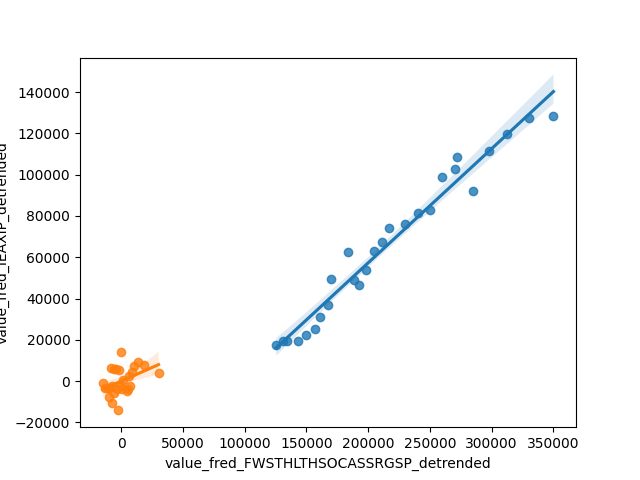
\includegraphics[scale = 0.9]{plots/plot_2026-08-29_detrended.png}
\caption{Detrended Regression Plot for 2026-08-29}
\end{figure}
\newpage
